\documentclass[12pt, a4paper, oneside]{ctexbook}
\usepackage{amsmath, amsthm, amssymb, bm, graphicx, hyperref, mathrsfs,}
\usepackage{newtxtext}
\usepackage[dvipsnames,svgnames]{xcolor}
\usepackage{tcolorbox}
\definecolor{dedcolor}{rgb}{0.77,0.72,0.65}

% 包含环境定义
% 定义可复用的tcolorbox环境类
% 定理环境
\newtcolorbox{theorembox}[1][]{
    colback=Emerald!10,
    colframe=cyan!40!black,
    title=\textbf{定理#1},
    fonttitle=\large,
    arc=3pt,
    boxrule=1pt
}

% 定义环境
\newtcolorbox{definitionbox}[1][]{
    title=\textbf{定义#1},
    colback=SeaGreen!10!CornflowerBlue!10,
    colframe=RoyalPurple!55!Aquamarine!100!,
    fonttitle=\large,
    arc=3pt,
    boxrule=1pt
}

% 引理环境
\newtcolorbox{lemmabox}[1][]{
    title=\textbf{引理#1},
    colback=Salmon!20,
    colframe=Salmon!90!Black,
    fonttitle=\large,
    arc=3pt,
    boxrule=1pt
}

% 推论环境
\newtcolorbox{corollarybox}[1][]{
    title=\textbf{推论#1},
    colback=OldLace,
    colframe=dedcolor,
    fonttitle=\large,
    arc=3pt,
    boxrule=1pt
}

% 证明环境
\newtcolorbox{proofbox}[1][]{
    colback=JungleGreen!10!Cerulean!15,
    colframe=CornflowerBlue!60!Black,
    fonttitle=\large,
    arc=3pt,
    boxrule=1pt,
    before upper={\textbf{证明#1}}
} 

\title{{\Huge{\textbf{现代机器人学笔记}}}}
\author{hanzhuchen666}
\date{2025年7月29日}
\linespread{1.5}
\newtheorem{theorem}{定理}[section]
\newtheorem{definition}[theorem]{定义}
\newtheorem{lemma}[theorem]{引理}
\newtheorem{corollary}{推论}
\newtheorem{example}{例}
\newtheorem{proposition}{命题}

\begin{document}

\maketitle

\pagenumbering{roman}
\setcounter{page}{1}

\begin{center}
    \Huge\textbf{前言}
\end{center}~\

前言内容

注:本文所使用一些图示如下

% 使用封装后的环境类
\begin{theorembox}
这是定理
\end{theorembox}

\begin{definitionbox}
这是定义
\end{definitionbox}

\begin{lemmabox}
这是引理
\end{lemmabox}

\begin{corollarybox}
这是推论
\end{corollarybox}

\begin{proofbox}
这是证明
\end{proofbox}
~\\
\begin{flushright}
    \begin{tabular}{c}
        hanzhuchen666\\
        
    \end{tabular}
\end{flushright}

\newpage
\pagenumbering{Roman}
\setcounter{page}{1}
\tableofcontents
\newpage
\setcounter{page}{1}
\pagenumbering{arabic}

\chapter{现代控制论基础}
\section{状态空间方程与线性系统}
\begin{equation*}
	\begin{cases}
		x[k+1] = Ax[k] + Bu[k]\\
		y[k] = Cx[k] + Du[k]
	\end{cases}
\end{equation*}
\subsection{连续系统到离散系统相互转换}
线性情况下
\begin{equation*}
  \begin{cases}
  	\dot{x} = A_cx + B_cu\\
  	y = C_cx + D_cu
  \end{cases}
\end{equation*}
可以转换为
\begin{equation*}
  \begin{cases}
  	x[k+1] = A_dx[k] + B_du[k]\\
  	y[k] = C_dx[k] + D_du[k]
  \end{cases}
\end{equation*}
其中
\begin{gather*}
 A_d = I + A_c\Delta t\\
 B_d = B_c \Delta t \\
 C_d = C_c\\
 D_d = D_c 
\end{gather*}
\subsubsection{前向欧拉法}
\subsubsection{后向欧拉法}
\subsubsection{其他方法}
\section{非线性近似为线性系统}
\section{最小二乘推导}
测量公式,$\theta \in R^n$ 是隐藏参数,$ v \in R^m $ 是测量噪声
\begin{equation}
  y = g(\theta) + v
\end{equation}

问题定义:
\begin{equation}
  \min{\theta \in \Theta}J(\theta) = min \Vert y - g(\theta) \Vert ^2
\end{equation}
线性最小二乘:$g(\theta) = H \theta $
利用简单的数学计算
\begin{theorembox}
	if $f(x) = Ax$, then $\nabla f(x) = A$
\end{theorembox}
\begin{theorembox}
	if $f(x) = x^TAx$, then $\nabla f(x) = A^Tx+Ax$
\end{theorembox}
可以证明
\begin{theorembox}
	如果$H\in R^{m\times n}$列满秩,则存在解$\theta = (H^TH)^{-1}H^Ty$ 
\end{theorembox}
\section{逆矩阵}
\begin{theorembox}
	针对矩阵$A \in R^{m\times n}$,若A列满秩,则矩阵左逆为$A_{left}^{-1} = (A^TA)^{-1}A^T$,满足$A_{left}^{-1}A = I_{n \times n}$。
\end{theorembox}


\section{伪逆矩阵Moore-Penrose逆}
摩尔-彭罗斯逆的应用场景:
\begin{itemize}
  \item 最小二乘问题::线性回归等问题中,当系数矩阵不是方阵时,摩尔-彭罗斯逆可以用来求解最小二乘解。
  \item 欠定方程组::对于方程组的解不唯一的情况,摩尔-彭罗斯逆可以找到一个具有最小范数的解。
  \item 矩阵的秩的计算::摩尔-彭罗斯逆可以用来确定一个矩阵的秩。
  \item 信号处理和图像处理::在这些领域中,摩尔-彭罗斯逆可以用于去噪、滤波等任务。
  \item 控制理论::用于设计控制器,特别是当系统模型是非方阵时。
\end{itemize}
摩尔-彭罗斯逆的性质:
\begin{itemize}
  \item 唯一性::对于任意一个矩阵,其摩尔-彭罗斯逆是唯一的。
  \item 广义逆::如果一个矩阵是可逆的,那么它的摩尔-彭罗斯逆就是它的普通逆矩阵。
  \item 满足Penrose 方程::摩尔-彭罗斯逆满足四个特定的Penrose 方程,这些方程定义了摩尔-彭罗斯逆的性质。
\end{itemize}



\section{投影矩阵}

\subsection{最小二乘应用与例子}
\begin{enumerate}
  \item 可以用作求解线性方程组的最小
二乘根,使得解误差的而范数最小
  \item 可以通过构造方程组来进行系统参数辨识
\end{enumerate}
\section{稳定性、可控性和可观性}
\section{状态反馈/输出反馈控制设计}
\section{状态空间跟踪控制器设计}
\section{卡尔曼滤波原理}
\subsection{扩展卡尔曼滤波}




\chapter{函数最优化问题求解方式}
\section{原始牛顿法}
\section{雅可比矩阵和Hessian矩阵}
\section{高斯-牛顿法}
\section{拟牛顿法}
\subsection{Levenberg-Marquardt algorithm, LM}
\subsection{Davidon-Fletcher-Powell algoritm DFP}
\subsection{Broyden–Fletcher–Goldfarb–Shanno algorithm BFGS}


\chapter{最优控制}
\section{LQR}
\subsection{iLQR}
\subsection{DDP}

\chapter{轨迹优化}
\section{概述}
\section{直接法}
\subsection{Single Shooting}
\subsection{Multiple Shooting}
\subsection{Collocation Method}
\section{间接法}






\chapter{动力学基础}
\chapter{基于旋量理论的动力学}
\section{符号约定}
\section{}
\chapter{基于约束的动力学方程求解}

\chapter{矩阵分解}\label{MathTools:chap:matrix_decomposition}
\section{LU分解}\label{MathTools:sec:lu_decomposition}
\section{QR分解及HouseHolder方法}\label{MathTools:sec:qr_decomposition}
\subsection{HouseHolder方法}\label{MathTools:sec:householder}
\section{SVD奇异值分解}\label{MathTools:sec:svd}
% todo : SVD奇异值分解搬运
\begin{theorembox}
	$A = U\Sigma V^T$,其中$U$和$V^T$是酉矩阵,$\Sigma$是对角线矩阵
\end{theorembox}
\subsubsection{SVD分解应用于PCA主成份分析}
https://www.cnblogs.com/daniel-D/p/3218063.html
\chapter{矩阵的逆及其求解方式}\label{MathTools:chap:matrix_inverse}
\section{LU分解求解对称正定矩阵的逆}\label{MathTools:sec:lu_inverse}
\section{QR分解求解右伪逆}\label{MathTools:sec:qr_pseudoinverse}
\section{SVD分解求广义逆}\label{MathTools:sec:svd_pseudoinverse}



\chapter{函数最优化问题求解方式}\label{MathTools:chap:optimization}
\section{原始牛顿法}\label{MathTools:sec:newton_method}
\section{雅可比矩阵和Hessian矩阵}\label{MathTools:sec:jacobian_hessian}
\section{高斯-牛顿法}\label{MathTools:sec:gauss_newton}
\section{拟牛顿法}\label{MathTools:sec:quasi_newton}
\subsection{Levenberg-Marquardt algorithm, LM}\label{MathTools:sec:lm}
\subsection{Davidon-Fletcher-Powell algoritm DFP}\label{MathTools:sec:dfp}
\subsection{Broyden–Fletcher–Goldfarb–Shanno algorithm BFGS}\label{MathTools:sec:bfgs}

\chapter{未分类}
\section{条件数}
条件数是线性方程组Ax=b的解对b中的误差或不确定度的敏感性的度量。数学定义为矩阵A的条件数等于A的范数与A的逆的范数的乘积,即cond(A)=‖A‖·‖A-1‖,对应矩阵的3种范数,相应地可以定义3种条件数。

matlab 里面运算函数:cond(A,2)或cond(A):2范数

一个极端的例子,当A奇异时,条件数为无穷,这时即使不改变b,x也可以改变。奇异的本质原因在于矩阵有0特征值,x在对应特征向量的方向上运动不改变Ax的值。如果一个特征值比其它特征值在数量级上小很多,x在对应特征向量方向上很大的移动才能产生b微小的变化,这就解释了为什么这个矩阵为什么会有大的条件数,事实上,正规阵在二范数下的条件数就可以表示成 abs(最大特征值/最小特征值)。——摘自百度百科

在计算机编程环境中,数据都是有浮点类型表示,精度有限,存在干扰,因此在解线性方程的时候都会存在误差。

\subsection{病态矩阵与条件数}
% todo : 条件数与病态矩阵
https://www.cnblogs.com/daniel-D/p/3219802.html
\subsubsection{与特征值和SVD的关系}
\subsubsection{病态矩阵的处理方法}
5. 病态矩阵处理方法
真正的自由是建立在规范的基础上的。病态矩阵解集的不稳定性是由于解集空间包含了自由度过大的方向,解决这个问题的关键就是将这些方向去掉,而保留 scaling 较大的方向,从而把解集局限在一个较小的区域内。在上面的讨论中, A 矩阵的特征向量不一定正交,不适合做新基, SVD 分解正好分解出了正交基,可以选前 k 个 $v^T$ 向量作为正交基。

比如,现在只选取前一个 (0.707, 0.707) 方向作为基,解集局限咋 y = x 这条直线上。直观的解释就是, A 矩阵的两个列向量过于类似,我们就可以将它们等同看待,第一次 b = (1000, 0), 解集是(0.5, 0.5), 第二次 b = (1000, 0.001), 解集还是 (0.5, 0.5).

总结起来,解决 A 病态就是将解集限定在一组正交基空间内,即对于坐标 y, 选择 k 个正交基 Zk,解决问题:$$\min_{y}\Vert AZ_ky - b \Vert ^2$$
这个就是 reduce-rank model. 具体方法有 truncated SVD 和 Krylov subspace method。
\section{带约束的最小范数解问题}
问题定义:
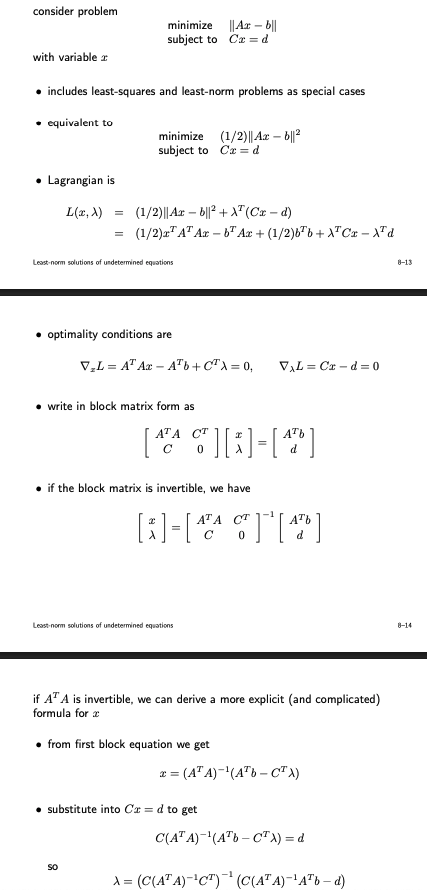
\includegraphics{MathTools/assets/rinv_with_constraints.png}
\begin{theorembox}
	$x = (A^TA)^{-1}(A^Tb-C^T(C(A^TA)^{-1}C^T)^{-1}(C(A^TA)^{-1}A^Tb-d))$
\end{theorembox}
\section{酉矩阵}
https://zh.wikipedia.org/wiki/%E9%85%89%E7%9F%A9%E9%98%B5
\subsection{图形中的稀疏表示}
% todo : 图形中的稀疏表示



\end{document}